% !TEX TS-program = pdflatex
% =====================================================================
%  AIMS 5790 Final Defence Presentation  --  Yuxiao Zhao  --  April 2026
%  25 min talk + 10 min Q&A
%
%  SPEAKER NOTES  (how to present):
%    Option A (recommended):  Install pympress   (pip install pympress)
%      pympress slides.pdf    -> projector shows slide, your screen shows notes
%    Option B:  Compile TWO PDFs
%      1)  pdflatex -jobname=slides presentation.tex       (notes PDF, for you)
%      2)  comment out \setbeameroption line, recompile     (clean PDF, for projector)
%    Option C:  Any PDF viewer with dual-monitor "presenter view"
%
%  VIDEOS:
%    Click any video thumbnail to play externally.
%    Video .mp4 files must be in the same folder as this PDF.
% =====================================================================
\documentclass[10pt,aspectratio=169]{beamer}

% ----- speaker notes control -----
% For slides-only PDF (used for PPTX generation), comment out the next 2 lines:
%\usepackage{pgfpages}
%\setbeameroption{show notes on second screen=right}
% The primary deliverable is now the PPTX file with embedded videos.

% ----- theme -----
\usetheme{Madrid}
\usecolortheme{seahorse}
\useinnertheme{circles}
\setbeamertemplate{navigation symbols}{}
\setbeamertemplate{caption}[numbered]
\setbeamerfont{frametitle}{size=\large,series=\bfseries}
\setbeamerfont{title}{size=\Large,series=\bfseries}

% ----- packages -----
\usepackage[T1]{fontenc}
\usepackage{lmodern}
\usepackage{graphicx}
\usepackage{booktabs}
\usepackage{array}
\usepackage{amsmath,amssymb}
\usepackage{multirow}
\usepackage{tikz}
\usepackage{xcolor}
\usepackage{multimedia}
\usepackage{hyperref}
\usetikzlibrary{arrows.meta,positioning,shapes.geometric,fit,backgrounds,
                 calc,decorations.pathmorphing}

% ----- colours -----
\definecolor{cuhkpurple}{RGB}{112,48,160}
\definecolor{accent}{RGB}{220,120,40}
\definecolor{good}{RGB}{30,140,60}
\definecolor{alertred}{RGB}{200,40,40}
\definecolor{lightbg}{RGB}{245,242,250}
\setbeamercolor{structure}{fg=cuhkpurple}
\setbeamercolor{frametitle}{fg=white,bg=cuhkpurple}
\setbeamercolor{title}{fg=cuhkpurple}
\setbeamercolor{block title}{bg=cuhkpurple!85!black,fg=white}
\setbeamercolor{block body}{bg=cuhkpurple!8}
\setbeamercolor{block title alerted}{bg=alertred!90!black,fg=white}
\setbeamercolor{block body alerted}{bg=alertred!8}
\setbeamercolor{block title example}{bg=good!80!black,fg=white}
\setbeamercolor{block body example}{bg=good!8}

\newenvironment{keybox}[1][Key Insight]{%
  \begin{exampleblock}{#1}}{\end{exampleblock}}

% slide number
\setbeamertemplate{footline}{%
  \hfill\insertframenumber/\inserttotalframenumber\hspace*{6pt}\vspace{2pt}}

% ----- title -----
\title[Legged Manipulation -- B2Z1]{%
  Legged Manipulation with RoboDuet:\\[2pt]
  Adapting the B2Z1 Quadruped--Arm Platform\\
  for End-Effector Reaching and Object Approaching}
\subtitle{AIMS 5790 --- Final Project Defence}
\author[Yuxiao Zhao]{Yuxiao Zhao \\ {\small Student ID: 1155246057}}
\institute[CUHK]{%
  MSc in Artificial Intelligence\\
  The Chinese University of Hong Kong\\[4pt]
  {\normalsize\textit{Supervisor: Prof.\ Fei Chen}}}
\date{April 2026}

% =====================================================================
\begin{document}

% =====================================================================
%  TITLE
% =====================================================================
\begin{frame}[plain]
  \titlepage
\end{frame}
\note{
Good morning/afternoon, professors. My name is Yuxiao Zhao. Today I will
present my AIMS 5790 final project: adapting the RoboDuet legged manipulation
framework from the small Unitree Go1 robot to the much larger B2 platform.
I will walk you through the background, the complete pipeline, and the
current simulation results. The presentation will take about 25 minutes,
and I am happy to answer questions afterwards.
}

% =====================================================================
%  OUTLINE
% =====================================================================
\begin{frame}{Outline}
  \tableofcontents[hideallsubsections]
  \vspace{8pt}
  {\small\color{gray}
   Presentation: $\sim$25 min \hfill
   Q\&A: $\sim$10 min}
\end{frame}
\note{
Here is the outline. I will start with a brief background so everyone is
on the same page. Then I show the full project pipeline --- a flowchart
of every step from hardware to final result. After that: hardware and
software setup, the RoboDuet method, training details, and finally demos.
}

% #####################################################################
%  SECTION 1 --- BACKGROUND  (3 min)
% #####################################################################
\section{Background and Motivation}

\begin{frame}{What Is a ``Loco-Manipulator''?}
  \begin{columns}[T]
    \begin{column}{0.55\textwidth}
      \textbf{Robots need two capabilities:}
      \begin{enumerate}
        \item \textbf{Locomotion} --- moving around\\
              (walking, climbing stairs)
        \item \textbf{Manipulation} --- interacting with objects\\
              (picking up, pushing, pressing)
      \end{enumerate}

      \vspace{6pt}
      A \textbf{loco-manipulator} combines both:\\
      a walking robot with a robotic arm on its back.

      \vspace{6pt}
      \begin{keybox}[Analogy]
        Think of a person carrying a tray of drinks while walking
        through a crowd --- your legs and arms must \emph{cooperate}.
      \end{keybox}
    \end{column}
    \begin{column}{0.42\textwidth}
      \centering
      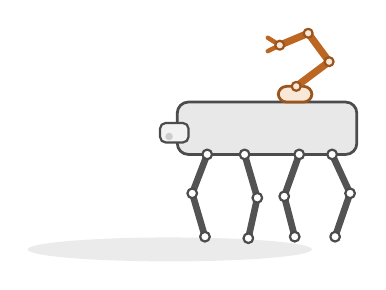
\begin{tikzpicture}[scale=0.95,transform shape,
          line cap=round,line join=round,
          limb/.style={draw=gray!65!black,line width=2.4pt},
          joint/.style={circle,draw=gray!60!black,fill=white,line width=0.8pt,inner sep=1.3pt}]
        \fill[black!8] (-1.35,-1.45) ellipse (1.9 and 0.16);
        \filldraw[rounded corners=4pt,fill=gray!18,draw=gray!60!black,line width=1pt]
          (-1.25,-0.18) rectangle (1.15,0.52);
        \filldraw[rounded corners=2pt,fill=gray!10,draw=gray!60!black,line width=0.8pt]
          (-1.48,-0.02) rectangle (-1.10,0.24);
        \fill[gray!40] (-1.36,0.06) circle (0.05);

        \coordinate (lfh) at (-0.85,-0.18);
        \coordinate (lfk) at (-1.05,-0.70);
        \coordinate (lff) at (-0.88,-1.28);
        \coordinate (lrh) at (0.82,-0.18);
        \coordinate (lrk) at (1.06,-0.70);
        \coordinate (lrf) at (0.86,-1.28);
        \coordinate (rfh) at (-0.35,-0.18);
        \coordinate (rfk) at (-0.18,-0.76);
        \coordinate (rff) at (-0.30,-1.30);
        \coordinate (rrh) at (0.38,-0.18);
        \coordinate (rrk) at (0.18,-0.74);
        \coordinate (rrf) at (0.32,-1.28);

        \draw[limb] (lfh) -- (lfk) -- (lff);
        \draw[limb] (lrh) -- (lrk) -- (lrf);
        \draw[limb] (rfh) -- (rfk) -- (rff);
        \draw[limb] (rrh) -- (rrk) -- (rrf);
        \foreach \p in {lfh,lfk,lff,lrh,lrk,lrf,rfh,rfk,rff,rrh,rrk,rrf}
          \node[joint] at (\p) {};

        \filldraw[rounded corners=3pt,fill=accent!18,draw=accent!70!black,line width=1pt]
          (0.10,0.52) rectangle (0.55,0.73);
        \coordinate (ab) at (0.34,0.73);
        \coordinate (ae) at (0.78,1.06);
        \coordinate (aw) at (0.50,1.44);
        \coordinate (ag) at (0.12,1.28);
        \draw[draw=accent!85!black,line width=2.6pt] (ab) -- (ae) -- (aw) -- (ag);
        \draw[draw=accent!85!black,line width=1.6pt] (ag) -- ++(-0.16,0.10);
        \draw[draw=accent!85!black,line width=1.6pt] (ag) -- ++(-0.16,-0.08);
        \foreach \p in {ab,ae,aw,ag}
          \node[circle,fill=accent!18,draw=accent!70!black,line width=0.8pt,inner sep=1.2pt] at (\p) {};
      \end{tikzpicture}\\[4pt]
      {\scriptsize Generic quadruped--arm platform schematic}
    \end{column}
  \end{columns}
\end{frame}
\note{
Let me start by explaining what we are building.
A loco-manipulator is a robot that can both walk and interact with objects.
Think of Unitree's quadruped robots --- they walk very well, but they cannot
pick anything up. If you mount a robotic arm on top, you get a system that
can both move AND interact.
The analogy: imagine carrying a tray of drinks through a crowd.
Your legs handle the walking, your arms handle the tray, and your brain
coordinates them so you do not spill.
}

\begin{frame}{Why Is This Hard?}
  \begin{columns}[T]
    \begin{column}{0.52\textwidth}
      When the arm moves, three things go wrong:
      \begin{itemize}
        \item The \textbf{centre of gravity shifts}\\
              $\rightarrow$ the robot may tip over
        \item The arm creates \textbf{reaction forces}\\
              $\rightarrow$ legs must compensate
        \item Walking vibrations \textbf{shake the arm}\\
              $\rightarrow$ end-effector misses its target
      \end{itemize}

      \vspace{6pt}
      \textbf{Classical approaches (and their limits):}
      \begin{enumerate}
        \item One giant controller $\rightarrow$ too many parameters
        \item Two independent controllers $\rightarrow$ they ignore each other
      \end{enumerate}
    \end{column}
    \begin{column}{0.46\textwidth}
      \centering
      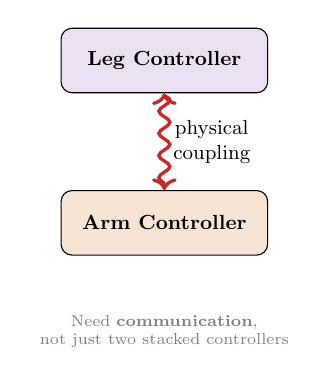
\begin{tikzpicture}[scale=0.82,transform shape,
          box/.style={draw,rounded corners,minimum width=3.2cm,
                      minimum height=1cm,font=\small\bfseries}]
        \node[box,fill=cuhkpurple!15] (leg) {Leg Controller};
        \node[box,fill=accent!20,below=1.5cm of leg] (arm) {Arm Controller};
        \draw[<->,very thick,alertred,decorate,
              decoration={snake,amplitude=2pt,segment length=8pt}]
              (leg) -- node[right,black,font=\small,align=center]
              {physical\\coupling} (arm);
        \node[below=0.8cm of arm,text width=4cm,align=center,
              font=\scriptsize\color{gray}]
          {Need \textbf{communication},\\not just two stacked controllers};
      \end{tikzpicture}
    \end{column}
  \end{columns}
\end{frame}
\note{
When the arm moves, it shifts the centre of gravity.
If the legs do not react, the robot tips over.
You might think: just train two separate controllers. But if they do not
communicate, the arm will surprise the legs every time it moves.
We need the two controllers to cooperate.
That is exactly what RoboDuet does --- I will explain shortly.
}

\begin{frame}{Reinforcement Learning and PPO}
  \begin{columns}[T]
    \begin{column}{0.52\textwidth}
      \textbf{Reinforcement Learning (RL):}
      \begin{itemize}
        \item An \textbf{agent} (robot) takes \textbf{actions}
              (joint torques) in an \textbf{environment} (simulator)
        \item After each action it receives a \textbf{reward}
        \item Over millions of trials, it learns a \textbf{policy}
              $\pi$: sensor data $\rightarrow$ actions
      \end{itemize}

      \vspace{4pt}
      \textbf{PPO} (Proximal Policy Optimisation):
      \begin{enumerate}
        \item Let 4\,096 robots act for 24 steps each
        \item Compute: ``was this action better or worse than average?''
        \item Update the policy, but \textbf{clip} the update so it
              never changes too drastically
      \end{enumerate}
      \vspace{2pt}
      {\small
      $L^{\text{CLIP}} = \mathbb{E}\big[
        \min\!\big(r_t\hat{A}_t,\;
              \text{clip}(r_t, 1{-}\epsilon, 1{+}\epsilon)\hat{A}_t\big)
      \big]$}
    \end{column}
    \begin{column}{0.46\textwidth}
      \centering
      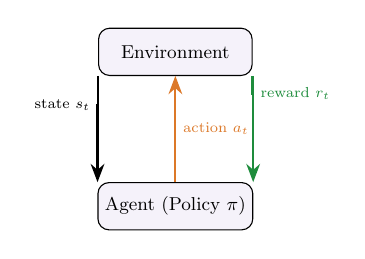
\begin{tikzpicture}[scale=0.75,transform shape,
          node distance=1.2cm,>=Stealth,
          block/.style={draw,rounded corners,fill=lightbg,
                        minimum width=2.6cm,minimum height=0.8cm,
                        font=\small}]
        \node[block] (env) {Environment};
        \node[block,below=1.8cm of env] (agent) {Agent (Policy $\pi$)};
        \draw[->,thick] (env.south west) -- ++(0,-0.5) -|
          node[pos=0.25,left,font=\scriptsize]{state $s_t$} (agent.north west);
        \draw[->,thick,good] (env.south east) -- ++(0,-0.3) -|
          node[pos=0.25,right,font=\scriptsize,good]{reward $r_t$} (agent.north east);
        \draw[->,thick,accent] (agent.north) --
          node[right,font=\scriptsize,accent]{action $a_t$} (env.south);
      \end{tikzpicture}
      \vspace{6pt}\\
      {\scriptsize The RL loop:\\observe $\rightarrow$ act $\rightarrow$ reward $\rightarrow$ improve}

      \vspace{6pt}
      \begin{keybox}[Why simulation?]
        {\scriptsize GPU simulator: \textbf{4096 robots in parallel} ---
        years of experience in hours.}
      \end{keybox}
    \end{column}
  \end{columns}
\end{frame}
\note{
For those less familiar with RL: the robot tries actions, receives rewards,
and gradually learns.
The specific algorithm is PPO --- the standard for robotics RL.
PPO's key idea: clip the policy update so it never changes too drastically
in one step. This makes training stable.
We do everything in simulation. NVIDIA IsaacGym runs 4096 robots on one
GPU. In 3 hours we accumulate about 1.5 years of real-robot experience.
}

% #####################################################################
%  SECTION 2 --- PIPELINE OVERVIEW  (2 min)
% #####################################################################
\section{Project Goal and Pipeline}

\begin{frame}{Project Goal in One Sentence}
  \centering
  \vspace{0.8cm}
  {\Large\bfseries
    Take the RoboDuet framework (designed for the \textcolor{cuhkpurple}{small Go1})\\[6pt]
    and make it work on the \textcolor{accent}{much larger B2} quadruped.}

  \vspace{1cm}
  \begin{columns}[c]
    \begin{column}{0.42\textwidth}
      \centering
      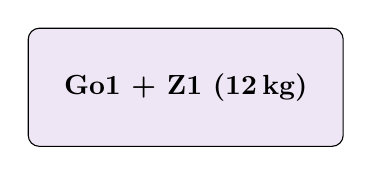
\begin{tikzpicture}
        \node[draw,rounded corners,fill=cuhkpurple!12,
              minimum width=4cm,minimum height=1.5cm,font=\bfseries]
              {Go1 + Z1 (12\,kg)};
      \end{tikzpicture}
    \end{column}
    \begin{column}{0.1\textwidth}
      \centering {\Huge$\boldsymbol{\Rightarrow}$}
    \end{column}
    \begin{column}{0.42\textwidth}
      \centering
      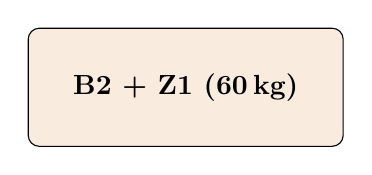
\begin{tikzpicture}
        \node[draw,rounded corners,fill=accent!15,
              minimum width=4cm,minimum height=1.5cm,font=\bfseries]
              {B2 + Z1 (60\,kg)};
      \end{tikzpicture}
    \end{column}
  \end{columns}

  \vspace{0.7cm}
  {\small 5$\times$ heavier body, different joint limits, different control gains\\
   $\Rightarrow$ every parameter must be re-tuned; pre-trained weights are useless.}
\end{frame}
\note{
This is the core of my project in one sentence.
RoboDuet was built and validated on the Unitree Go1 --- 12 kilograms.
My task: migrate it to the Unitree B2 --- 60 kilograms, 5 times heavier.
Every single parameter had to be changed. Pre-trained Go1 weights are
completely useless on B2.
}

\begin{frame}{End-to-End Pipeline Overview}
  \centering
  \vspace{2pt}
  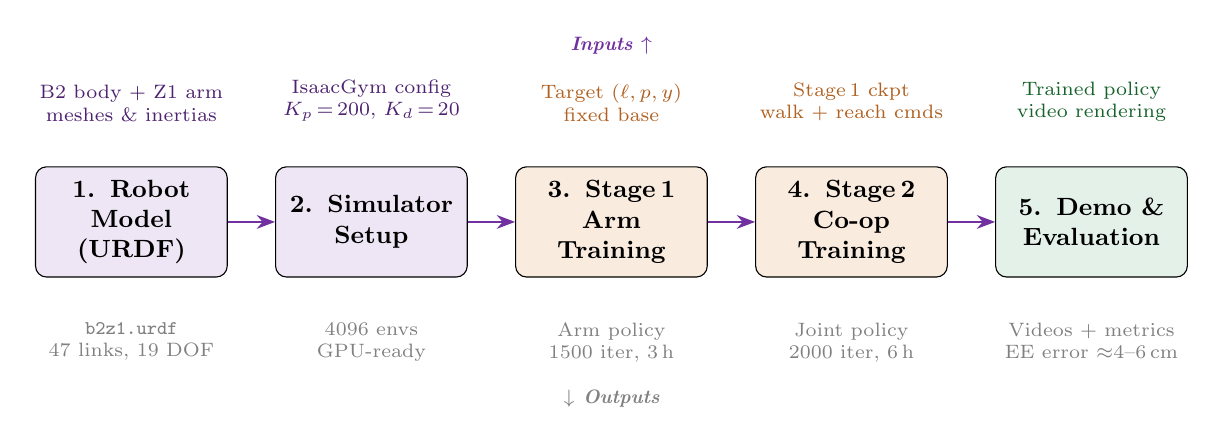
\begin{tikzpicture}[
      >=Stealth,
      stage/.style={draw, rounded corners=4pt, minimum height=1.4cm,
                    minimum width=2.4cm, text width=2.2cm, align=center,
                    font=\small\bfseries},
      io/.style={font=\scriptsize, text width=2.4cm, align=center},
      arr/.style={->, thick, cuhkpurple},
    ]
    % --- boxes ---
    \node[stage, fill=cuhkpurple!12] (s1) {1. Robot Model\\(URDF)};
    \node[stage, fill=cuhkpurple!12, right=0.6cm of s1] (s2) {2. Simulator\\Setup};
    \node[stage, fill=accent!15, right=0.6cm of s2] (s3) {3. Stage\,1\\Arm Training};
    \node[stage, fill=accent!15, right=0.6cm of s3] (s4) {4. Stage\,2\\Co-op Training};
    \node[stage, fill=good!12, right=0.6cm of s4] (s5) {5. Demo \&\\Evaluation};

    % --- arrows ---
    \draw[arr] (s1) -- (s2);
    \draw[arr] (s2) -- (s3);
    \draw[arr] (s3) -- (s4);
    \draw[arr] (s4) -- (s5);

    % --- inputs (above) ---
    \node[io, above=0.45cm of s1, cuhkpurple!70!black]
      {B2 body + Z1 arm\\meshes \& inertias};
    \node[io, above=0.45cm of s2, cuhkpurple!70!black]
      {IsaacGym config\\$K_p\!=\!200$, $K_d\!=\!20$};
    \node[io, above=0.45cm of s3, accent!80!black]
      {Target $(\ell,p,y)$\\fixed base};
    \node[io, above=0.45cm of s4, accent!80!black]
      {Stage\,1 ckpt\\walk + reach cmds};
    \node[io, above=0.45cm of s5, good!70!black]
      {Trained policy\\video rendering};

    % --- outputs (below) ---
    \node[io, below=0.45cm of s1, gray]
      {\texttt{b2z1.urdf}\\47 links, 19 DOF};
    \node[io, below=0.45cm of s2, gray]
      {4096 envs\\GPU-ready};
    \node[io, below=0.45cm of s3, gray]
      {Arm policy\\1500 iter, 3\,h};
    \node[io, below=0.45cm of s4, gray]
      {Joint policy\\2000 iter, 6\,h};
    \node[io, below=0.45cm of s5, gray]
      {Videos + metrics\\EE error $\approx$4--6\,cm};

    % --- labels ---
    \node[above=1.3cm of s3, font=\scriptsize\itshape, cuhkpurple]
      {\textbf{Inputs} $\uparrow$};
    \node[below=1.3cm of s3, font=\scriptsize\itshape, gray]
      {$\downarrow$ \textbf{Outputs}};
  \end{tikzpicture}

  \vspace{8pt}
  {\small Each box is one project phase.
   Inputs are shown above; outputs below.\\
   The rest of this talk walks through each phase in detail.}
\end{frame}
\note{
This is the complete pipeline of my project, from start to finish.
Step 1: build the robot model by merging B2 body and Z1 arm into one URDF.
Step 2: configure the IsaacGym simulator with correct gains and environment count.
Step 3: Stage 1 training --- arm-only, body fixed, 1500 PPO iterations, about 3 hours.
Step 4: Stage 2 training --- legs and arm together, 2000 iterations, about 6 hours.
Step 5: generate demo videos and measure end-effector accuracy.
I will now walk through each of these in detail.
}

% #####################################################################
%  SECTION 3 --- HARDWARE & SOFTWARE  (5 min)
% #####################################################################
\section{Hardware and Software Setup}

\begin{frame}{Hardware Comparison: Go1 vs.\ B2}
  \begin{columns}[T]
    \begin{column}{0.56\textwidth}
      \begin{table}
        \small
        \begin{tabular}{l c c}
          \toprule
          & \textbf{Go1+Z1} & \textbf{B2+Z1} \\
          \midrule
          Body mass        & 12\,kg        & \textbf{60\,kg}  \\
          Payload          & 5\,kg         & \textbf{20\,kg}  \\
          Standing height  & 0.30\,m       & \textbf{0.55\,m} \\
          Leg DOFs         & 12            & 12              \\
          Arm DOFs         & 6 + 1 grip    & 6 + 1 grip      \\
          PD stiffness $K_p$ & 35          & \textbf{200}    \\
          PD damping $K_d$   & 0.5         & \textbf{20}     \\
          \bottomrule
        \end{tabular}
      \end{table}

      \vspace{4pt}
      \begin{alertblock}{Key challenge}
        Same arm, but the body underneath is 5$\times$ heavier and
        25\,cm taller. All mechanical parameters change.
      \end{alertblock}
    \end{column}
    \begin{column}{0.42\textwidth}
      \centering
      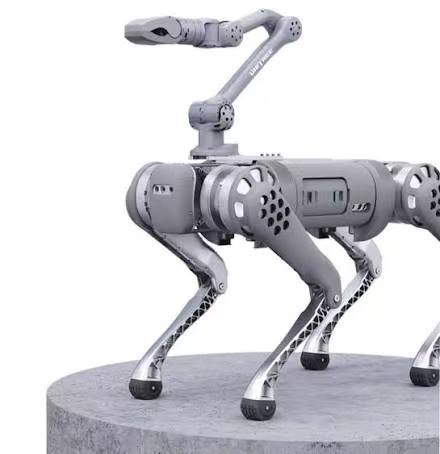
\includegraphics[width=0.95\linewidth]{b2z1_platform.jpg}\\[2pt]
      {\scriptsize Unitree B2 quadruped + Z1 arm}
    \end{column}
  \end{columns}
\end{frame}
\note{
The Go1 weighs 12 kg, stands 30 cm tall, uses joint stiffness Kp=35.
The B2 is 60 kg, stands 55 cm, needs Kp=200 --- nearly 6 times stiffer.
The arm is the same Z1 in both cases. But mounting it on a much heavier
body changes everything about the dynamics.
}

\begin{frame}{Software Stack: IsaacGym, URDF, and PyTorch}
  \begin{columns}[T]
    \begin{column}{0.50\textwidth}
      \textbf{What is IsaacGym?}
      \begin{itemize}
        \item NVIDIA's GPU physics simulator (2021)
        \item Rigid-body dynamics: gravity, contacts, motors
        \item Runs \textbf{4\,096 robots in parallel} on 1 GPU
        \item Data never leaves GPU: states $\to$ policy $\to$ physics
      \end{itemize}

      \vspace{4pt}
      \textbf{What is URDF?}
      \begin{itemize}
        \item Robot blueprint in XML: links, joints, masses, meshes
        \item Our \texttt{b2z1.urdf}: 47 links, 19 DOF, $\sim$41\,KB
        \item Created by merging B2 body + Z1 arm descriptions
      \end{itemize}
    \end{column}
    \begin{column}{0.48\textwidth}
      \textbf{Server environment}
      \begin{itemize}
        \item Remote RTX 4090 (24\,GB VRAM)
        \item Ubuntu 20.04
        \item PyTorch 2.4.1 + CUDA 12.1
        \item IsaacGym 1.0 Preview 4
      \end{itemize}

      \vspace{4pt}
      \textbf{Automation}
      \begin{itemize}
        \item Automated upload / run / poll scripts
        \item \texttt{restart\_demo\_only.py} --- one-click deploy
        \item SSH-based log monitoring
      \end{itemize}

      \vspace{4pt}
      \begin{keybox}[Speedup]
        {\small 3 hours training $\approx$ \textbf{1.5 years} of
        real-robot experience}
      \end{keybox}
    \end{column}
  \end{columns}
\end{frame}
\note{
IsaacGym is NVIDIA's GPU physics simulator designed for RL.
Everything stays on the GPU --- no CPU-GPU transfer bottleneck.
A URDF file is the blueprint of the robot in XML.
Our b2z1.urdf was created by merging the B2 body and Z1 arm descriptions.
All training was done on a remote server with an RTX 4090.
I wrote automation scripts so I can upload code, launch training, and
poll logs without manual SSH --- this saved a lot of time.
Important: IsaacGym must be imported BEFORE PyTorch, or it crashes.
This is undocumented and took time to figure out.
}

\begin{frame}{Control Gain Tuning ($K_p$, $K_d$)}
  \textbf{PD control:}
  $\;\tau = K_p \cdot (q_{\text{target}} - q) \;-\; K_d \cdot \dot{q}$

  \vspace{6pt}
  \begin{columns}[T]
    \begin{column}{0.52\textwidth}
      \begin{table}
        \centering\small
        \begin{tabular}{c c l}
          \toprule
          $K_p$ & $K_d$ & \textbf{Result on B2} \\
          \midrule
          35  & 0.5 & Legs too weak, collapses \\
          100 & 5   & Stands but wobbles \\
          150 & 15  & Stable, slight drift \\
          \textbf{200} & \textbf{20} & \textbf{Stable 20\,s+} \\
          \bottomrule
        \end{tabular}
      \end{table}

      \vspace{4pt}
      {\small 5$\times$ heavier $\Rightarrow$ $\sim$6$\times$ stiffer joints.\\
      Physically intuitive: heavier body = stiffer springs.}
    \end{column}
    \begin{column}{0.46\textwidth}
      \textbf{What I tuned:}
      \begin{enumerate}
        \item Default joint angles for 0.55\,m height\\
              (Go1 angles made B2 collapse)
        \item $K_p$ sweep: 35, 100, 150, 200
        \item $K_d$ scaled proportionally
        \item Arm stiffness kept at Z1 defaults\\
              (arm is the same hardware)
      \end{enumerate}
    \end{column}
  \end{columns}
\end{frame}
\note{
I did an empirical sweep of the PD gains.
At Kp equals 35, the Go1 value, the B2 collapses immediately because
the joints cannot support 60 kg.
At 200, stable for 20 seconds or more with the arm moving.
The scaling makes physical sense: 5 times heavier, roughly 6 times stiffer.
I also had to recompute the default joint angles. The Go1 angles make the
B2's longer legs fold incorrectly.
}

\begin{frame}{URDF Body Index Mapping and End-Effector Computation}
  \small
  The simulator stores all rigid bodies in a flat tensor. We must know
  which row corresponds to the gripper tip.

  \vspace{4pt}
  \begin{columns}[T]
    \begin{column}{0.48\textwidth}
      \textbf{Body index layout:}
      \begin{itemize}
        \item B2 trunk = index 0
        \item 12 leg links = indices 1--12
        \item Z1 arm links = indices 13--24
        \item \texttt{gripperStator} = index 24
        \item \texttt{gripperMover} = index \textbf{25}\\
              (last \emph{physical} body)
      \end{itemize}

      \vspace{4pt}
      \textbf{The catch:}\\
      \texttt{ee\_gripper\_link} (URDF link 47) has mass = 0\\
      $\Rightarrow$ IsaacGym \textbf{silently merges} it away!\\
      Cannot read its position from the tensor.
    \end{column}
    \begin{column}{0.50\textwidth}
      \textbf{Solution --- manual offset:}
      \[
        \mathbf{p}_{\text{ee}} = \mathbf{p}_{25}
          + 0.086\,\text{m} \;\times\; \hat{\mathbf{x}}_{\text{local}}(q_{25})
      \]
      \begin{itemize}
        \item Read position \& quaternion of body 25
        \item Rotate $[0.086, 0, 0]$ by the quaternion
        \item Add to get the true jaw-tip position
      \end{itemize}

      \vspace{6pt}
      \begin{keybox}[Why this matters]
        Without this offset, the ``end-effector position'' is
        8.6\,cm behind the actual gripper tip ---
        enough to miss a 6\,cm cube entirely.
      \end{keybox}
    \end{column}
  \end{columns}
\end{frame}
\note{
This is an important technical detail.
The URDF defines ee_gripper_link as the gripper tip. But it has zero mass.
IsaacGym silently removes zero-mass links from the physics tensor.
So when I try to read its position, I get garbage.
The fix: read gripperMover at body index 25, then add 0.086 metres
along its local X axis using the quaternion.
The 0.086 comes from the URDF joint offset definitions.
Without this correction, our end-effector position is 8.6 cm wrong ---
that is larger than the 6 cm cube we are trying to reach.
}

% #####################################################################
%  SECTION 4 --- ROBODUET METHOD  (5 min)
% #####################################################################
\section{The RoboDuet Method}

\begin{frame}{RoboDuet: Two Cooperating AI Agents}
  \begin{columns}[T]
    \begin{column}{0.5\textwidth}
      \textbf{Pan et al., 2024 (IEEE RA-L)}\\
      Open-source framework for legged manipulation.

      \vspace{6pt}
      \textbf{Core idea --- two cooperating policies:}
      \begin{itemize}
        \item $\pi_{\text{loco}}$ controls 12 \textbf{leg} joints
        \item $\pi_{\text{arm}}$ controls 6 \textbf{arm} joints + gripper
        \item They exchange \textbf{guidance signals} every step
      \end{itemize}

      \vspace{4pt}
      \begin{keybox}[Result on Go1+Z1]
        50\% better end-effector accuracy than a single policy.
        Validated in simulation and on real hardware.
      \end{keybox}
    \end{column}
    \begin{column}{0.48\textwidth}
      \centering
      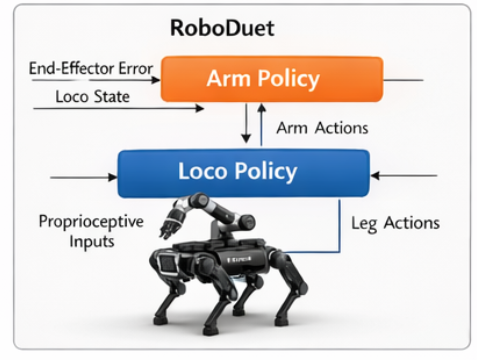
\includegraphics[width=\linewidth]{roboduet_overview.png}\\[2pt]
      {\scriptsize RoboDuet overview (Pan et al., 2024)}
    \end{column}
  \end{columns}
\end{frame}
\note{
RoboDuet was published in IEEE RA-L in 2024 by Pan et al.
Two separate neural network policies --- one for legs, one for arm ---
communicate at every control step.
The arm sends guidance signals to the legs: ``I am about to swing right,
please lean left.'' On Go1+Z1, this achieved 50 percent better accuracy
than a monolithic policy.
The code is open-source, which made it a good starting point.
}

\begin{frame}{Two-Stage Training Procedure}
  \centering
  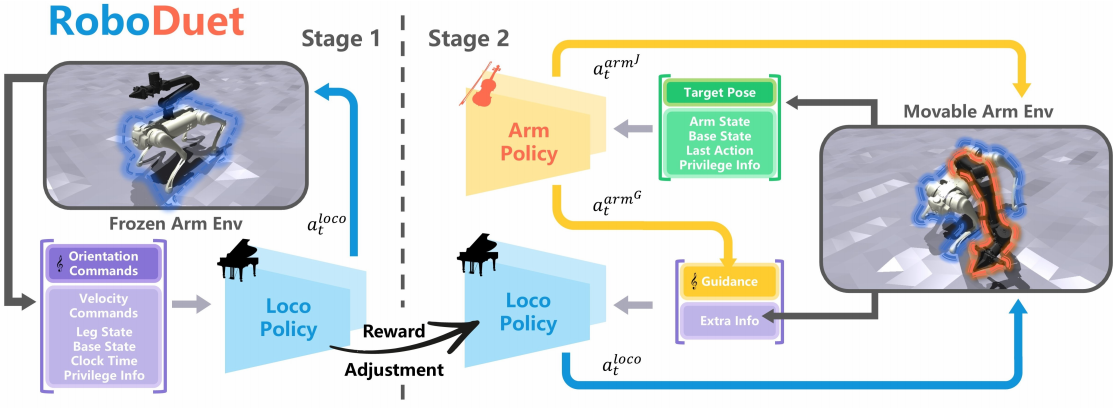
\includegraphics[width=0.82\textwidth]{roboduet_arch.png}\\[4pt]

  \begin{columns}[T]
    \begin{column}{0.48\textwidth}
      \textbf{Stage 1 --- Independent pre-training}
      \begin{itemize}
        \item Legs learn to walk with arm \textbf{frozen}
        \item Arm learns to reach with body \textbf{fixed}
        \item Each sub-task is simple $\Rightarrow$ fast convergence
      \end{itemize}
    \end{column}
    \begin{column}{0.48\textwidth}
      \textbf{Stage 2 --- Cooperated fine-tuning}
      \begin{itemize}
        \item Both policies \textbf{unfrozen}
        \item Communication channels activated
        \item Joint reward: walk well \emph{and} reach accurately
      \end{itemize}
    \end{column}
  \end{columns}
\end{frame}
\note{
Training happens in two stages.
Stage 1: train independently. Legs learn to walk with arm frozen.
Arm learns to reach with body bolted down. Simple tasks converge fast.
Stage 2: unfreeze both, train together. They learn to cooperate through
guidance signals. This curriculum is crucial --- training from scratch
with both active tends to diverge.
}

% ---- VIDEO: fixed-base arm demo ----
\begin{frame}{Stage 1 in Action: Fixed-Base Arm Reaching (Video)}
  \begin{columns}[c]
    \begin{column}{0.55\textwidth}
      \textbf{This is what Stage 1 arm training produces:}
      \begin{itemize}
        \item Robot body is \textbf{bolted to the ground}
        \item The arm explores different reach positions
        \item Controlled by spherical commands $(\ell, p, y)$
      \end{itemize}

      \vspace{6pt}
      This is the foundation --- the arm learns to move
      accurately \emph{before} we combine it with walking.

      \vspace{6pt}
      {\small\color{gray}Click the image to play.}
    \end{column}
    \begin{column}{0.43\textwidth}
      \centering
      \movie[externalviewer,poster]
        {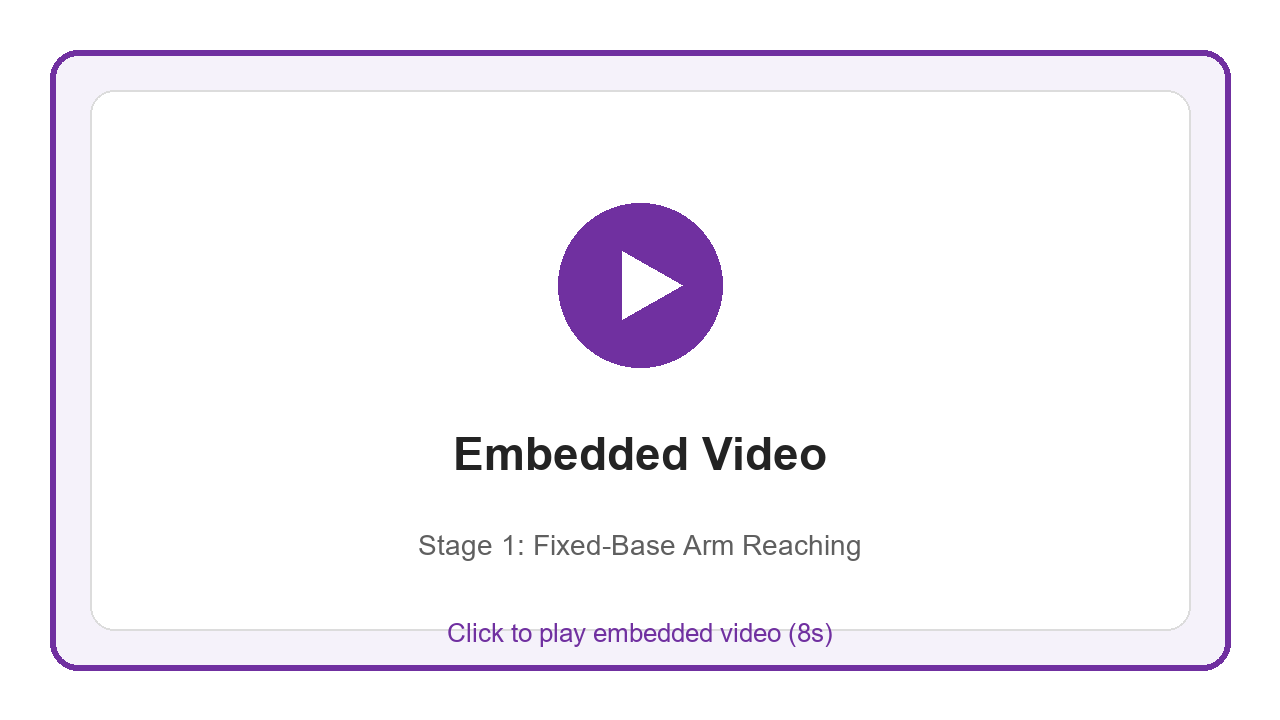
\includegraphics[width=\linewidth]{video_card_fixedbase.png}}
        {fixedbase_arm.mp4}\\[2pt]
      {\scriptsize Fixed-base arm reaching (8\,s)}
    \end{column}
  \end{columns}
\end{frame}
\note{
[CLICK TO PLAY VIDEO]
Here the body is fixed to the ground. The arm policy receives target
positions in spherical coordinates --- length, pitch, and yaw --- and
learns to reach those targets. You can see the arm smoothly transitioning
between different poses.
This is the checkpoint we start from for the grasp demo later.
}

\begin{frame}{How the Two Agents Communicate}
  \small
  \begin{table}
    \centering
    \begin{tabular}{>{\bfseries}l l p{6.2cm}}
      \toprule
      Signal & Direction & Plain-English Meaning \\
      \midrule
      $v_x, v_y, \omega$ & Human $\to$ Legs &
        ``Walk forward/sideways at this speed'' \\[3pt]
      $\ell, p, y$ & Human $\to$ Arm &
        ``Reach to this target (spherical coordinates)'' \\[3pt]
      Guidance & Arm $\to$ Legs &
        ``I am about to swing right --- lean left to compensate'' \\[3pt]
      Extra info & Legs $\to$ Arm &
        ``Body is tilted $3^{\circ}$ --- adjust your aim'' \\
      \bottomrule
    \end{tabular}
  \end{table}

  \vspace{4pt}
  \begin{keybox}[Why this matters]
    Without these guidance signals, the arm would surprise the legs
    every time it moves. The signals let the \textbf{legs prepare
    in advance} --- like a waiter bracing before lifting a heavy plate.
  \end{keybox}
\end{frame}
\note{
The human gives high-level commands: walk speed to legs, reach target to arm.
The key innovation: inter-agent communication.
Arm sends guidance to legs --- a preview of what it will do.
Legs send body state to arm --- tilt, height, velocity.
Think of a conductor coordinating two musicians.
}

\begin{frame}{Reward Design: What ``Good Behaviour'' Means}
  \scriptsize
  \begin{columns}[T]
    \begin{column}{0.55\textwidth}
      \begin{table}
        \centering
        \renewcommand{\arraystretch}{1.15}
        \begin{tabular}{l l c p{3.5cm}}
          \toprule
          \textbf{Category} & \textbf{Term} & \textbf{Wt} & \textbf{Description} \\
          \midrule
          \multirow{3}{*}{Loco}
            & vel tracking  & 1.0 & Match cmd $v_x, v_y, \omega_z$ \\
            & base height   & 1.0 & Keep CoM at target \\
            & orientation   & 0.5 & Penalise roll/pitch \\
          \midrule
          \multirow{2}{*}{Manip}
            & EE pos (lpy)  & 3.0 & Track target position \\
            & EE orient     & 1.0 & Track target orient \\
          \midrule
          \multirow{4}{*}{Reg}
            & torque        & $-0.01$ & Minimise motor effort \\
            & action rate   & $-0.05$ & Smooth motions \\
            & joint limits  & $-1.0$  & Avoid mech. limits \\
            & collision     & $-1.0$  & Avoid arm--body hit \\
          \bottomrule
        \end{tabular}
      \end{table}
    \end{column}
    \begin{column}{0.43\textwidth}
      \vspace{6pt}
      \textbf{Total reward:}
      \[
        r = \!\!\sum_{\text{loco}} w_i r_i
          + \!\!\sum_{\text{manip}} w_j r_j
          - \!\!\sum_{\text{reg}} w_k c_k
      \]

      \vspace{6pt}
      \textbf{Migration note:}\\
      Go1 weights caused \textbf{NaN gradients} on B2.
      The manipulation term (weight 3.0) produced huge
      initial errors on the larger arm.\\[3pt]
      Fix: reduce manipulation weight during early
      training, then restore.
    \end{column}
  \end{columns}
\end{frame}
\note{
The RL algorithm needs to know what good behaviour looks like.
Locomotion rewards: track velocity, keep body level and at the right height.
Manipulation rewards: end-effector position and orientation tracking.
Penalties: excessive torque, jerky motions, joint limits, collisions.
All weighted and summed. The manipulation position weight is 3.0, the highest.
A key migration challenge: these weights, tuned for Go1, caused numerical
explosions on B2 because the arm reaches further and creates larger errors.
I had to reduce the weight during early training to stabilise things.
}

% #####################################################################
%  SECTION 5 --- TRAINING & RESULTS  (5 min)
% #####################################################################
\section{Training Process and Results}

\begin{frame}{Training Setup and Hyperparameters}
  \begin{columns}[T]
    \begin{column}{0.50\textwidth}
      \textbf{Stage 1 --- Arm-only (fixed base)}
      \begin{itemize}
        \item 1\,500 PPO iterations, $\sim$3 hours
        \item Robot body is fixed; arm learns reaching
        \item Checkpoint: \texttt{ac\_weights\_last\_arm.pt}
      \end{itemize}

      \vspace{6pt}
      \textbf{Stage 2 --- Cooperated (standing + arm)}
      \begin{itemize}
        \item 2\,000 PPO iterations, $\sim$6 hours
        \item Both legs and arm active
        \item Communication channels enabled
      \end{itemize}
    \end{column}
    \begin{column}{0.48\textwidth}
      \centering
      \textbf{PPO Hyperparameters}\\[4pt]
      \small
      \begin{tabular}{l r l}
        \toprule
        \textbf{Param} & \textbf{Value} & \textbf{Note} \\
        \midrule
        Optimiser     & Adam     & Standard \\
        LR            & $10^{-3}$ & with decay \\
        Clip $\epsilon$ & 0.2    & PPO default \\
        $\gamma$      & 0.99     & Long horizon \\
        GAE $\lambda$ & 0.95     & Bias--var \\
        Entropy       & 0.005    & Exploration \\
        Envs          & 4\,096   & GPU parallel \\
        Epochs/update & 5        & Batch reuse \\
        Mini-batches  & 4        & Fits 24\,GB \\
        Steps/env     & 24       & Short rollouts \\
        \bottomrule
      \end{tabular}
    \end{column}
  \end{columns}
\end{frame}
\note{
Stage 1: 1500 PPO iterations, about 3 hours on RTX 4090.
Body fixed, arm learns reaching targets.
Stage 2: 2000 more iterations, about 6 hours.
Both policies active, cooperation is learned.
Hyperparameters are mostly standard PPO values.
4096 parallel environments to maximise GPU utilisation.
Mini-batch count of 4 fits the 24 GB VRAM budget.
}

\begin{frame}{Reward Curves}
  \begin{columns}[T]
    \begin{column}{0.48\textwidth}
      \centering
      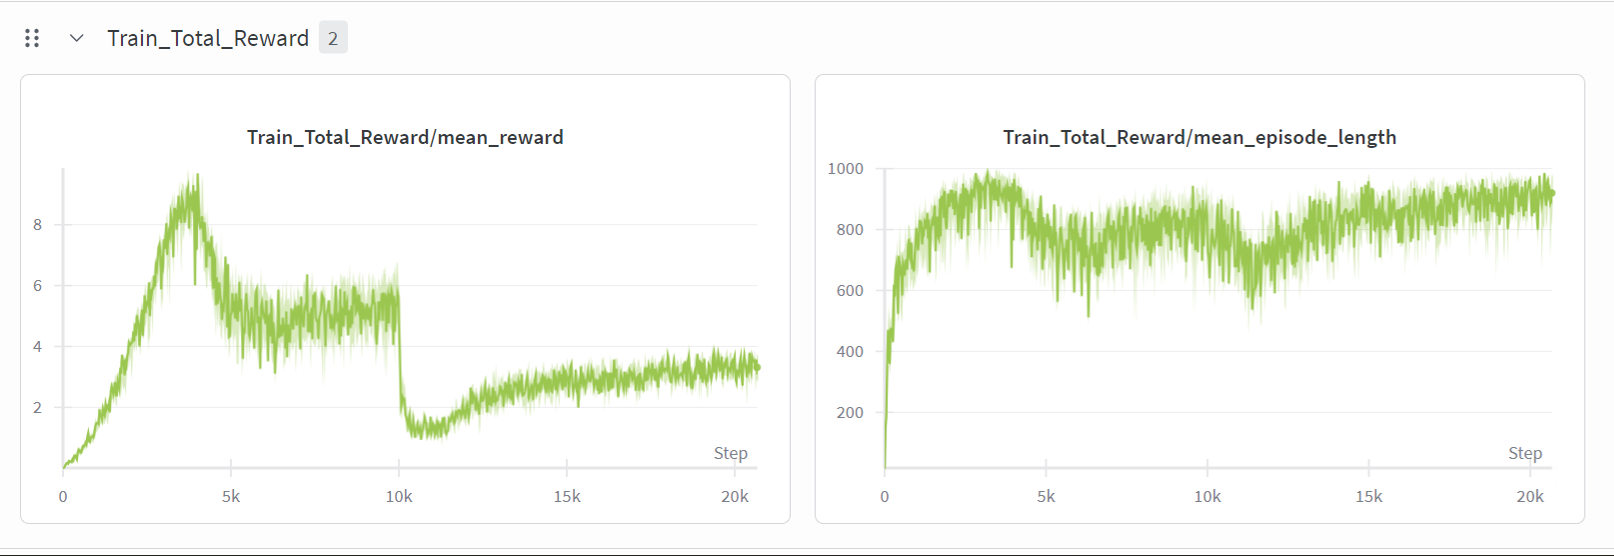
\includegraphics[width=\linewidth]{reward_total.png}\\[2pt]
      {\scriptsize Total return per training iteration}
    \end{column}
    \begin{column}{0.48\textwidth}
      \centering
      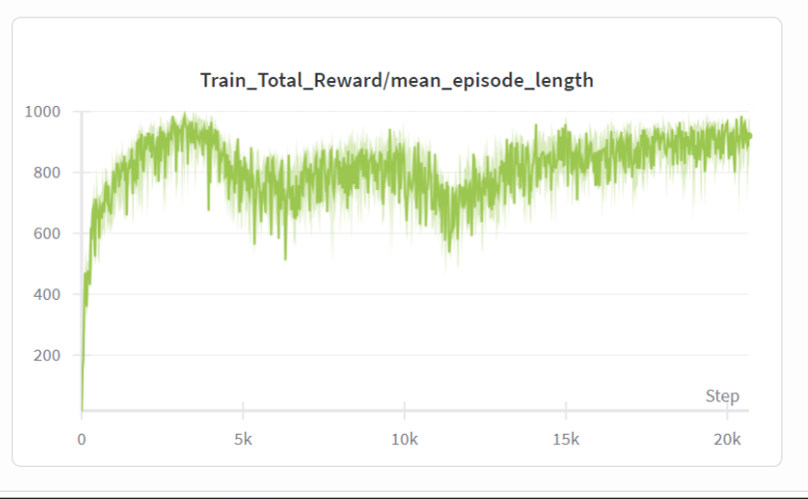
\includegraphics[width=\linewidth]{reward_train.png}\\[2pt]
      {\scriptsize Per-component reward breakdown}
    \end{column}
  \end{columns}

  \vspace{2pt}
  \begin{keybox}[Reading the curves]
    \footnotesize
    \begin{itemize}
      \setlength{\itemsep}{1pt}
      \item Monotonically increasing $\Rightarrow$ training is stable
      \item Locomotion reward saturates first --- walking is ``easier''
      \item Manipulation reward keeps improving --- more training would help
    \end{itemize}
  \end{keybox}
\end{frame}
\note{
Total return increases monotonically --- PPO training is stable.
This was NOT guaranteed on B2 since the reward weights needed careful
adjustment.
Locomotion saturates first: walking is simpler.
Manipulation keeps climbing: arm accuracy is still improving.
Longer training would likely improve manipulation further.
}

\begin{frame}{Quantitative Results}
  \begin{table}
    \centering
    \begin{tabular}{l c c c}
      \toprule
      \textbf{Demonstration} & \textbf{Base height (mean)}
        & \textbf{Height $\sigma$} & \textbf{EE position error} \\
      \midrule
      Fixed-base arm reach       & 0.55\,m (fixed) & 0.000\,m & 0.04\,m \\
      Standing + arm reach       & 0.52\,m         & 0.014\,m & 0.06\,m \\
      \bottomrule
    \end{tabular}
  \end{table}

  \vspace{6pt}
  \begin{columns}[T]
    \begin{column}{0.48\textwidth}
      \begin{keybox}[Stability]
        Standing demo: only $\pm$1.4\,cm height variation ---
        the B2 stays balanced while the arm moves.
      \end{keybox}
    \end{column}
    \begin{column}{0.48\textwidth}
      \begin{keybox}[Accuracy]
        4--6\,cm end-effector error ---
        the arm reliably reaches the vicinity of the target.
      \end{keybox}
    \end{column}
  \end{columns}
\end{frame}
\note{
Fixed base: 4 cm end-effector error.
Free standing: 6 cm error, body height varies by plus or minus 1.4 cm.
That 1.4 cm variation is very small for a 60 kg robot with a moving arm.
It shows the cooperative policy is working.
The 4-6 cm error is within the size of our 6 cm target cube.
}

\begin{frame}{Problems Encountered and Solved}
  \footnotesize
  \begin{table}
    \centering
    \renewcommand{\arraystretch}{1.25}
    \begin{tabular}{>{\raggedright\arraybackslash}p{4cm}
                    >{\raggedright\arraybackslash}p{8.5cm}}
      \toprule
      \textbf{What went wrong} & \textbf{Root cause and fix} \\
      \midrule
      Simulator crashes on startup &
      \texttt{isaacgym} must be imported \emph{before} PyTorch ---
      added a mandatory import guard \\

      Robot collapses immediately &
      Default joint angles designed for Go1's shorter legs;
      recomputed neutral pose for B2's 0.55\,m height \\

      Arm swings sideways instead of lifting &
      Arm commands use body-frame spherical coordinates;
      ``pitch'' rotates about body's local axis, not world-Z \\

      End-effector position reads as zero &
      \texttt{ee\_gripper\_link} is virtual (mass = 0); IsaacGym
      merges it away; used body 25 + 0.086\,m offset \\

      NaN gradients during training &
      Go1 reward weights too large for B2's bigger reach range;
      reduced manipulation weight in early iterations \\
      \bottomrule
    \end{tabular}
  \end{table}
\end{frame}
\note{
I want to be transparent about the problems encountered.
First: IsaacGym crashes if you import PyTorch before it. Undocumented.
Second: Go1 joint angles made B2 collapse. Had to recompute.
Third: increasing pitch makes the arm swing sideways, not up --- because
the spherical coordinates are relative to the body frame.
Fourth: ee_gripper_link has zero mass, so IsaacGym removes it silently.
Had to compute position from body 25 plus an 8.6 cm offset.
Fifth: NaN gradients because the larger B2 arm creates bigger initial errors,
amplified by Go1-tuned reward weights.
Each of these took significant debugging time.
}

% #####################################################################
%  SECTION 6 --- DEMOS  (4 min)
% #####################################################################
\section{Simulation Demonstrations}

% ---- VIDEO: standing demo ----
\begin{frame}{Demo 1: Standing Stability (Video)}
  \begin{columns}[c]
    \begin{column}{0.55\textwidth}
      \textbf{What you will see:}
      \begin{itemize}
        \item Robot remains upright throughout the shown clip
        \item Arm sweeps through reaching poses
        \item Visual focus: stable posture during arm motion
        \item This clip is selected to avoid collapse frames
      \end{itemize}

      \vspace{6pt}
      \textbf{This is the key Stage 2 result:}
      this selected demo segment highlights a stable upright posture
      while the arm changes pose.

      \vspace{6pt}
      {\small\color{gray}Click the image to play (20\,s).}
    \end{column}
    \begin{column}{0.43\textwidth}
      \centering
      \movie[externalviewer,poster]
        {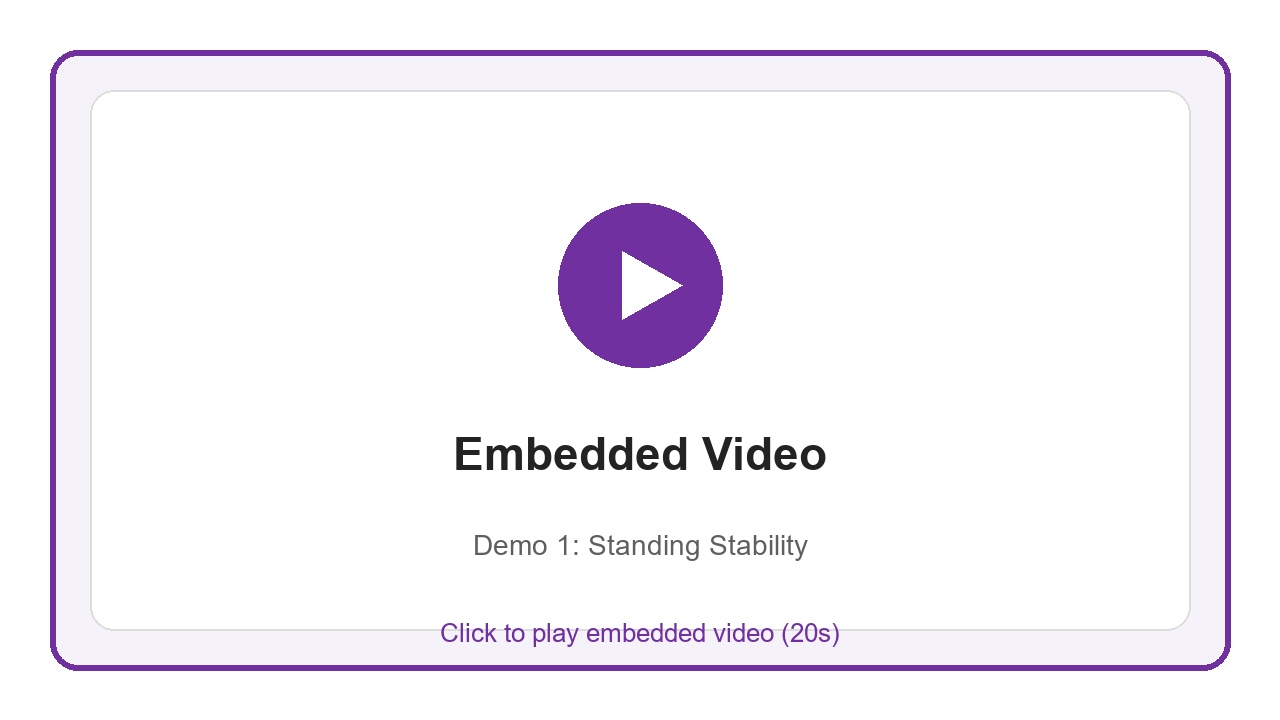
\includegraphics[width=\linewidth]{video_card_standing.png}}
        {standing_demo.mp4}\\[2pt]
      {\scriptsize B2+Z1 standing with arm motion}
    \end{column}
  \end{columns}
\end{frame}
\note{
[CLICK TO PLAY VIDEO]
This standing demo is a deliberately selected stable clip.
The main message here is simple: the robot remains upright while the arm moves.
I am using this clip for visual evidence of standing stability, without claiming
that every standing rollout is successful.
}

\begin{frame}{Standing Demo: Frame Sequence}
  \centering
  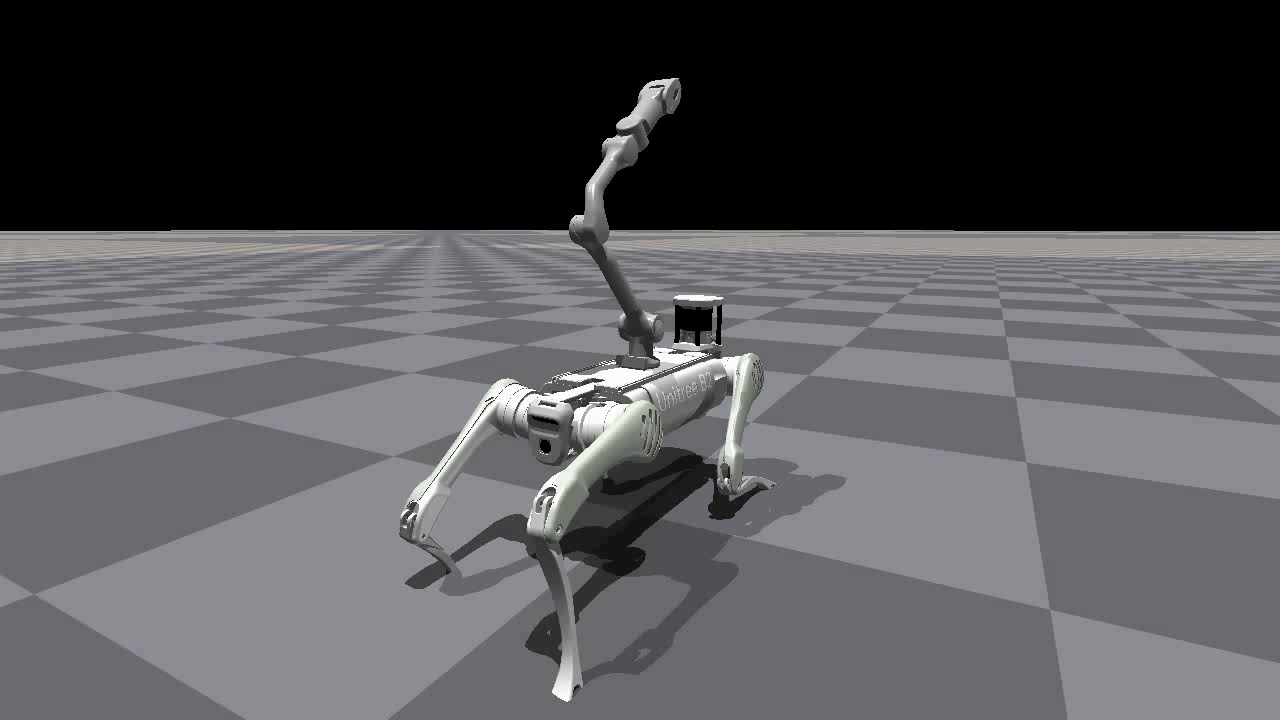
\includegraphics[width=0.23\linewidth]{stand_fixed_f000.png}\hfill
  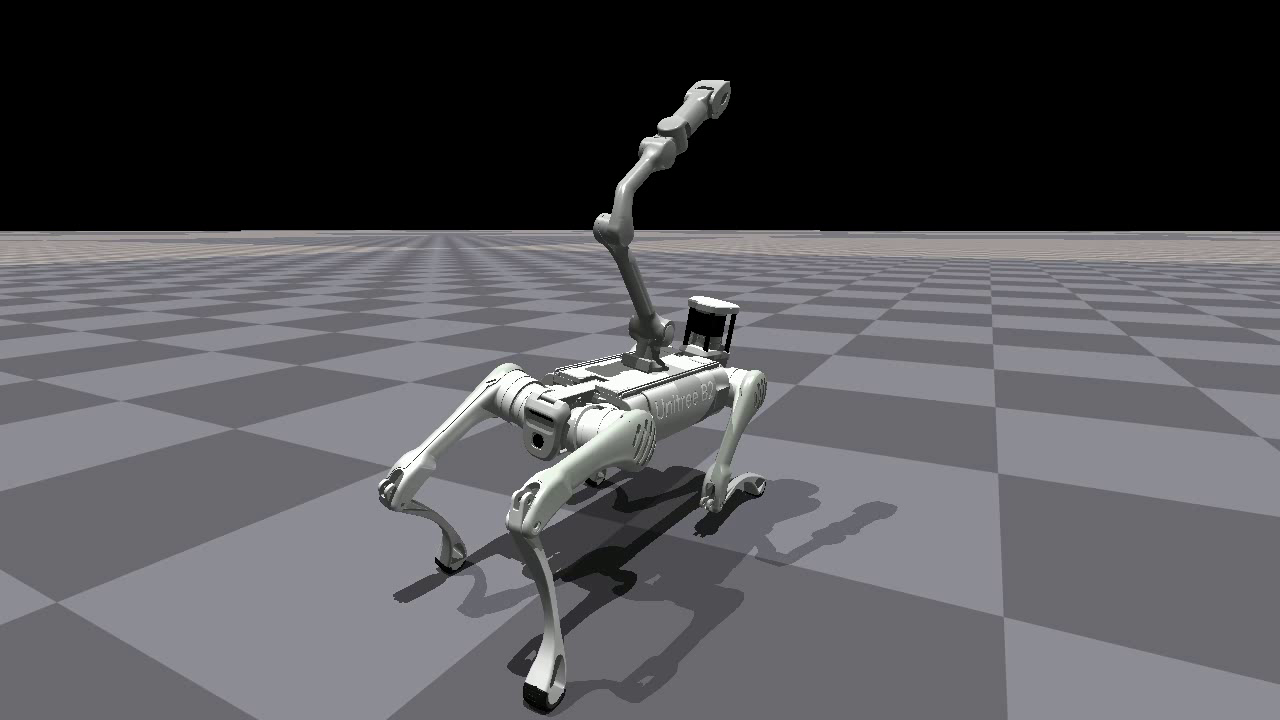
\includegraphics[width=0.23\linewidth]{stand_fixed_f100.png}\hfill
  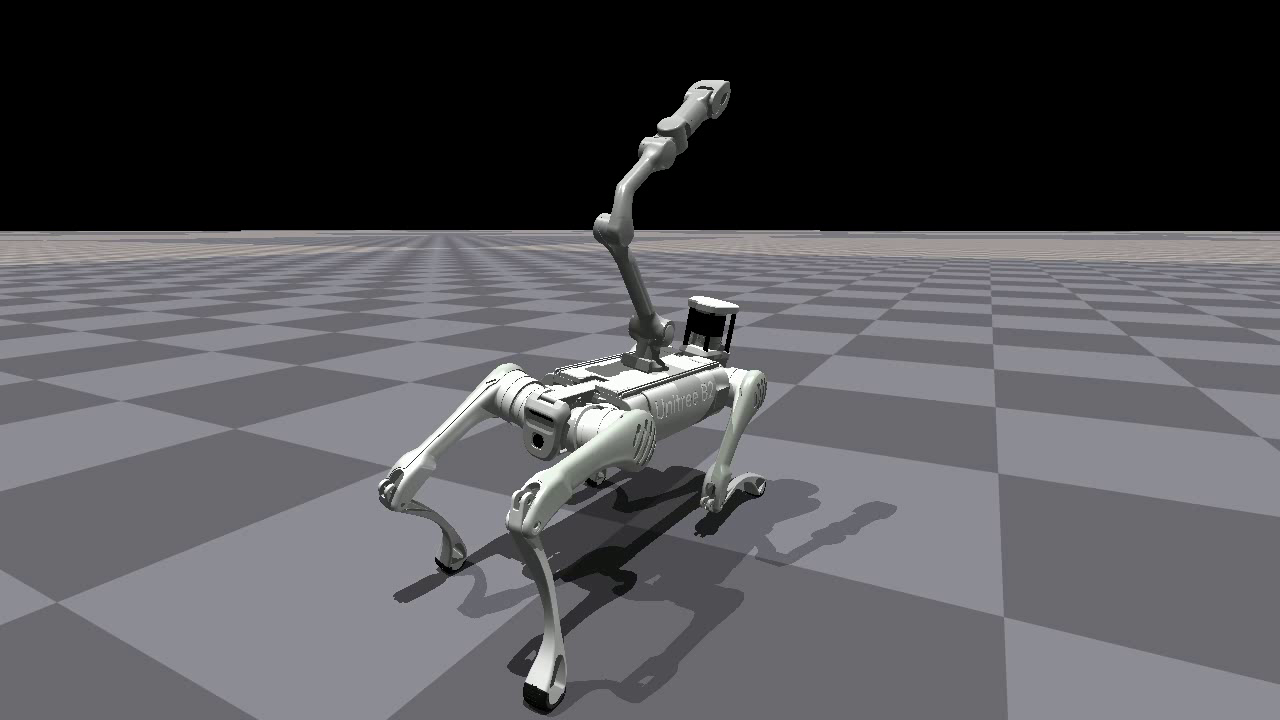
\includegraphics[width=0.23\linewidth]{stand_fixed_f300.png}\hfill
  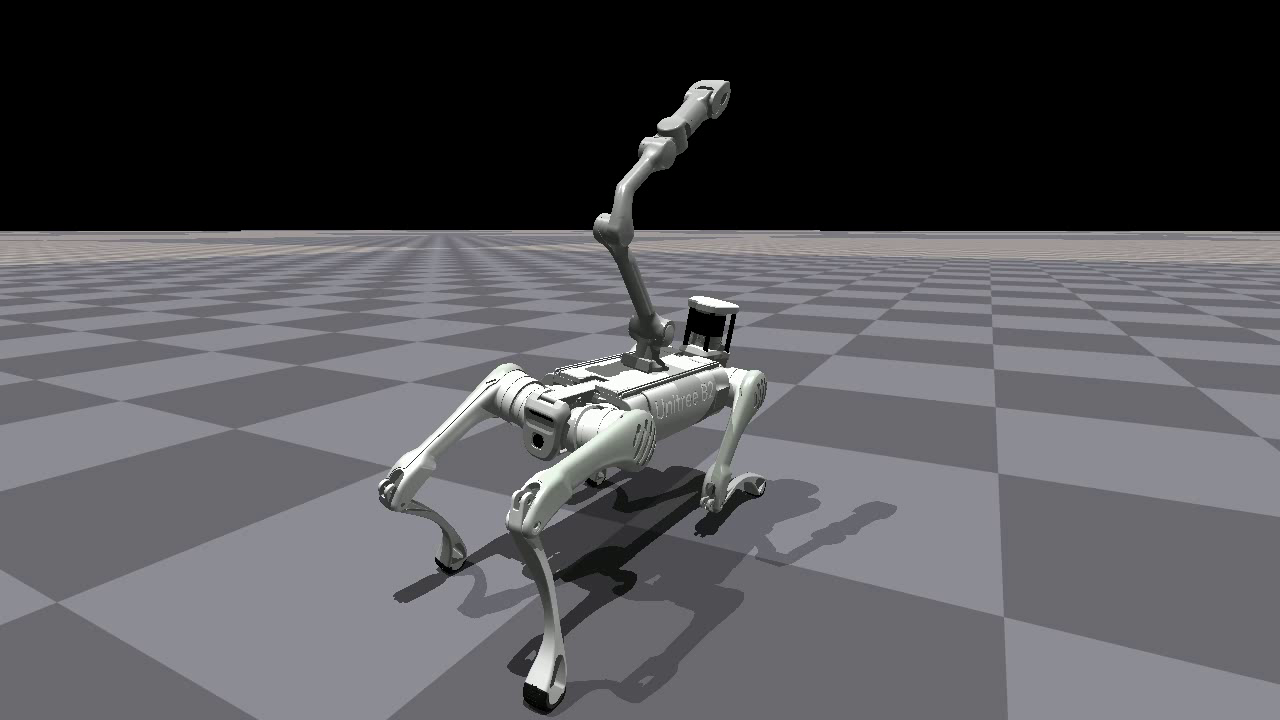
\includegraphics[width=0.23\linewidth]{stand_fixed_f500.png}

  \vspace{2pt}
  {\scriptsize
   $t = 0$\,s \hspace{2.1cm}
   $t = 4$\,s \hspace{2.2cm}
   $t = 8$\,s \hspace{2.2cm}
   $t = 12$\,s}

  \vspace{8pt}
  \begin{itemize}
    \item Four frames sampled from the updated stable standing clip
    \item The body posture remains upright across all shown frames
    \item This slide matches the embedded standing video on the previous page
  \end{itemize}
\end{frame}
\note{
Four frames are sampled from the updated stable standing clip.
At 0, 4, 8, and 12 seconds, the body remains upright while the arm changes pose.
The purpose of this sequence is to match the selected video and show a clean
non-collapsing standing example.
}

% ---- VIDEO: grasp approaching ----
\begin{frame}{Demo 2: Fixed-Base Grasp-and-Lift Demo (Video)}
  \textbf{Current status:} the fixed-base demo now shows
  \textbf{approach $\rightarrow$ close $\rightarrow$ lift}
  for a 6\,cm target cube.

  \vspace{4pt}
  \begin{columns}[T]
    \begin{column}{0.52\textwidth}
      \begin{itemize}
        \item Robot base is fixed for stable framing
        \item A 6\,cm green cube is placed at the calibrated
              end-effector position
        \item The arm reaches the calibrated cube position
        \item The gripper closes around the cube
        \item The cube is then lifted upward in the fixed-base demo
      \end{itemize}

      \vspace{4pt}
      \begin{alertblock}{Honest status}
        This is a \textbf{fixed-base scripted demo result}.\
        A robust learned grasp-and-lift policy under standing or walking
        is \textbf{still not solved}.
      \end{alertblock}
    \end{column}
    \begin{column}{0.46\textwidth}
      \centering
      \movie[externalviewer,poster]
        {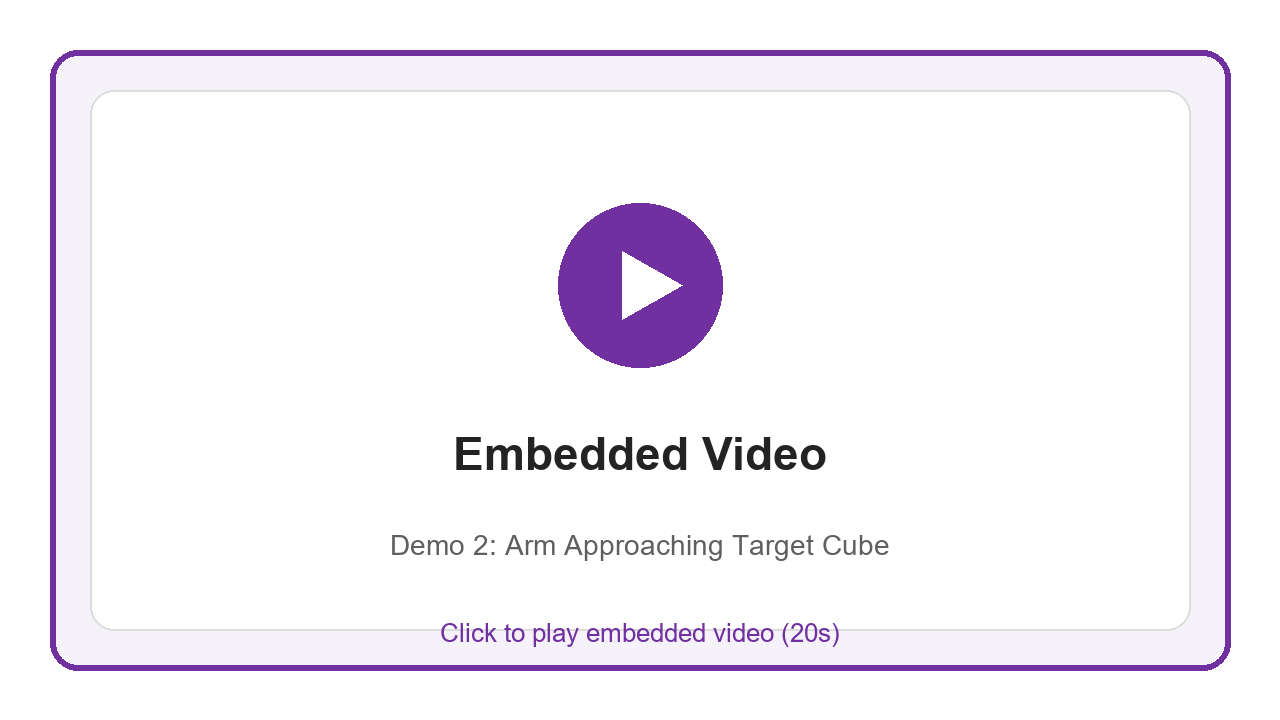
\includegraphics[width=\linewidth]{video_card_grasp.png}}
        {grasp_demo.mp4}\\[2pt]
      {\scriptsize Fixed-base grasp-and-lift demo (20\,s)}
    \end{column}
  \end{columns}
\end{frame}
\note{
[CLICK TO PLAY VIDEO]
Now the most important demo. The green cube is 6 cm, placed at the
calibrated end-effector position.
In this updated fixed-base sequence, the arm reaches the cube,
the gripper closes, and the cube is lifted.
But I want to be precise: this is not yet a robust learned grasp policy
under the full floating-base RoboDuet setting.
}

\begin{frame}{Fixed-Base Grasp Demo: Frame-by-Frame}
  \centering
  \begin{tabular}{ccc}
    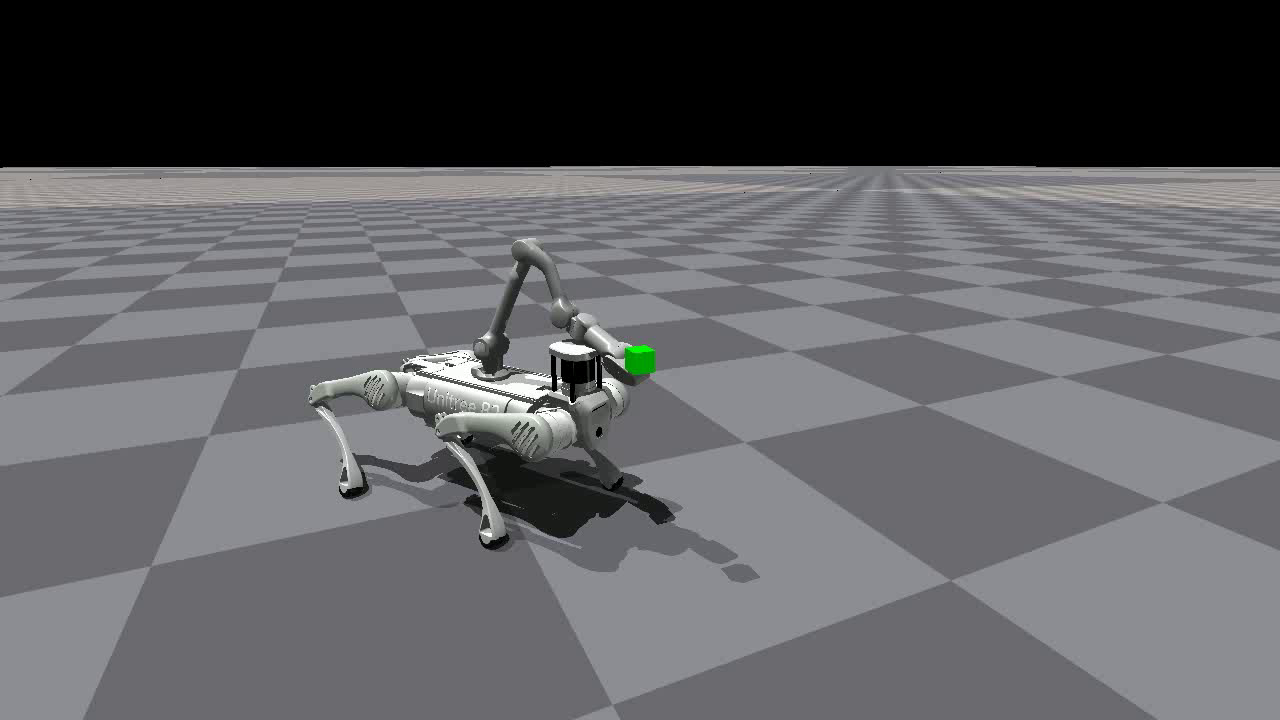
\includegraphics[width=0.30\linewidth]{demo_frame0.png} &
    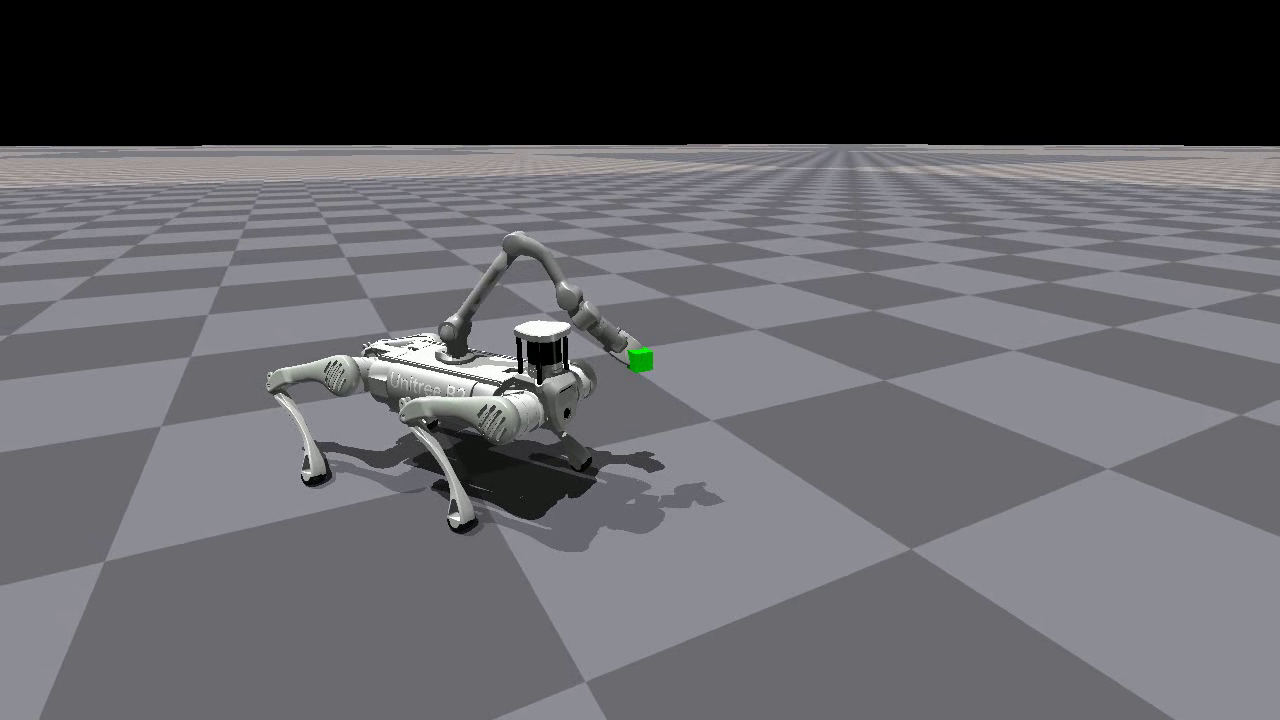
\includegraphics[width=0.30\linewidth]{demo_reach.png}  &
    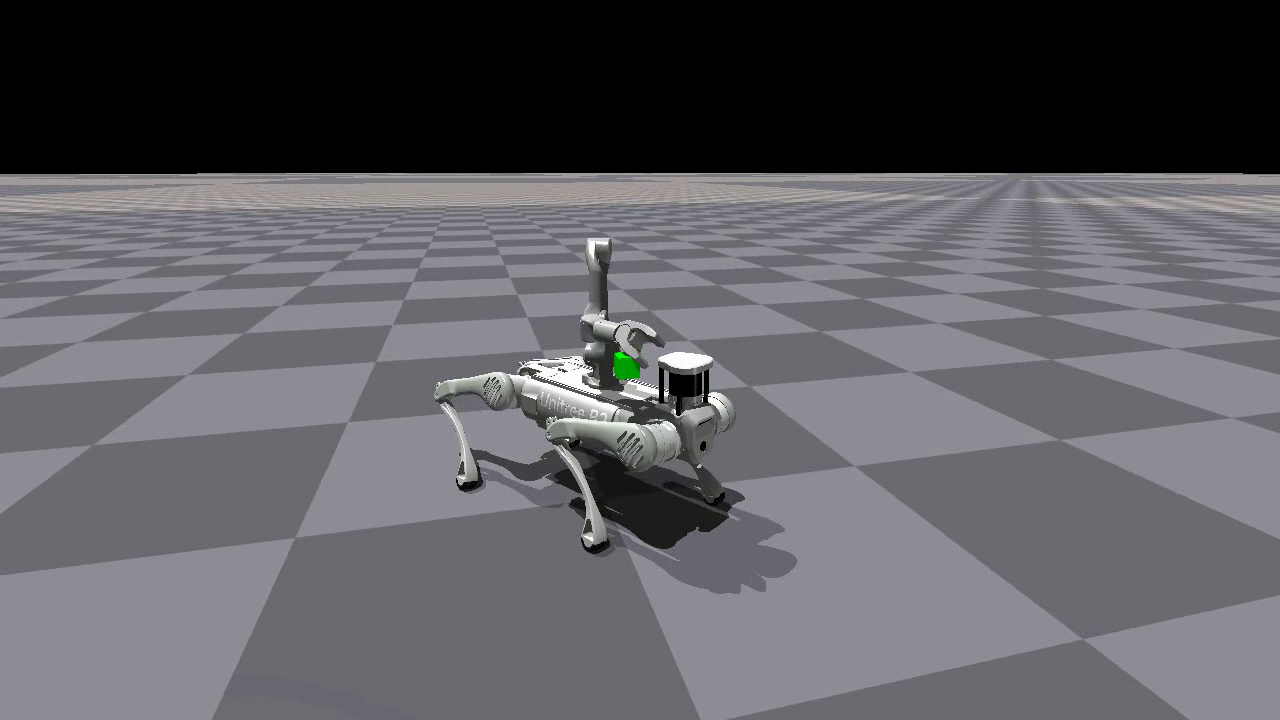
\includegraphics[width=0.30\linewidth]{demo_grasp.png}  \\[2pt]
    {\scriptsize \textcolor{gray}{$t = 0$\,s --- arm retracted}} &
    {\scriptsize \textcolor{cuhkpurple}{$t = 10.7$\,s --- gripper closing}} &
    {\scriptsize \textcolor{good}{$t = 18.7$\,s --- cube lifted}} \\
  \end{tabular}

  \vspace{8pt}
  \begin{itemize}
    \item Frame 0: arm is retracted, cube sits on the ground in front
    \item Frame 320: gripper closes around the cube
    \item Frame 560: cube has moved upward with the gripper --- lift shown
  \end{itemize}

  \vspace{4pt}
  \begin{keybox}[What this proves]
    Accurate reaching on B2+Z1 is good enough to support a fixed-base
    grasp-and-lift style demonstration on a 6\,cm target cube.
  \end{keybox}
\end{frame}
\note{
Frame 0: arm retracted, cube on the ground.
Frame 320: gripper closes around the cube.
Frame 560: the cube has been lifted upward.
This shows that the fixed-base demo pipeline can now produce a full
approach-close-lift sequence.
}

\begin{frame}{Why General Learned Lifting Is Still Hard}
  The arm command uses \textbf{spherical coordinates} $(\ell, p, y)$
  relative to the \emph{body frame}:
  \begin{columns}[T]
    \begin{column}{0.48\textwidth}
      \begin{itemize}
        \item $\ell$ = reach length
        \item $p$ = pitch (relative to body axis)
        \item $y$ = yaw (left/right)
      \end{itemize}

      \vspace{6pt}
      \textbf{Core issue:} increasing $p$ from 0.25 to 0.50
      makes the arm swing \emph{sideways}
      ($\sim$35\,cm in Y), not lift vertically.

      \vspace{4pt}
      ``Pitch'' rotates about the body's local axis,
      not world-Z.
    \end{column}
    \begin{column}{0.50\textwidth}
      \textbf{Implication for robust grasping:}
      \begin{itemize}
        \item A general vertical lift \textbf{cannot} be achieved by
              simply changing the pitch command
        \item Need either:
          \begin{enumerate}
            \item Remap commands to world-frame Z
            \item Scripted trajectory for lift phase
            \item Retrain with a lift-specific reward
          \end{enumerate}
      \end{itemize}

      \vspace{4pt}
      {\small This is why a general learned lift policy is still
      an open problem, even though the fixed-base demo can show lifting.}
    \end{column}
  \end{columns}
\end{frame}
\note{
This explains why general learned lifting is still hard.
The arm command uses spherical coordinates relative to the body frame.
When I increase pitch, the arm swings sideways, not upward.
This is because pitch rotates about the body's local axis, which is
roughly horizontal when the arm is extended forward.
There are three possible fixes, all listed here. This is the main
technical blocker for turning the fixed-base demo into a robust learned
grasp-and-lift capability.
}

% #####################################################################
%  SECTION 7 --- STATUS & FUTURE WORK  (3 min)
% #####################################################################
\section{Current Status and Future Work}

\begin{frame}{What Has Been Achieved}
  \begin{enumerate}
    \setlength{\itemsep}{7pt}
    \item \textbf{Reproduced} RoboDuet end-to-end and verified the published
          Go1+Z1 behaviour

    \item \textbf{Migrated} the entire pipeline to B2+Z1
          ($5\times$ heavier), retuning URDF, PD gains, reward weights,
          and initial pose from scratch

    \item \textbf{Trained} new policy checkpoints on B2+Z1:
          arm-only reaching (fixed base) and standing with arm reaching

    \item \textbf{Demonstrated} accurate reaching on a small target,
          and a fixed-base visual grasp-and-lift sequence in simulation

    \item Delivered a \textbf{reproducible codebase}
          with automated training and video-generation scripts
  \end{enumerate}
\end{frame}
\note{
Summary of achievements:
One, reproduced RoboDuet and verified it.
Two, migrated everything to B2+Z1 --- new URDF, gains, rewards, pose.
Three, trained two working checkpoints from scratch.
    Four, demonstrated successful reaching and a fixed-base visual grasp-and-lift demo.
Five, reproducible code with automation scripts.
}

\begin{frame}{What Is Not Yet Done (Honest Assessment)}
  \begin{alertblock}{Limitations}
    \begin{itemize}
      \item \textbf{Robust learned grasping not yet working} ---
            the fixed-base demo can show close + lift, but reliable learned grasping
            under standing or walking is still being debugged

      \item \textbf{General learned lifting not yet working} ---
            spherical coordinates do not map cleanly to vertical lift;
            requires a different control or training approach

      \item \textbf{Walking + manipulation not yet stable} ---
            Stage 2 works for standing, but walking while reaching
            introduces too much perturbation

      \item \textbf{No sim-to-real transfer} ---
            real B2 costs $\sim$\$30\,000; domain randomisation
            (mass, friction, motor delay, sensor noise)
            not yet implemented
    \end{itemize}
  \end{alertblock}
\end{frame}
\note{
Being completely transparent.
First, robust learned grasping: the fixed-base visual demo works,
but the full learned policy does not yet grasp reliably under disturbance.
Second, general learned lifting: the spherical command system cannot lift vertically.
Third, walking plus manipulation: too much perturbation for current policy.
Fourth, no sim-to-real. B2 costs 30 thousand dollars, and domain
randomisation is not yet implemented. A 60 kg robot with an untested
policy is also genuinely dangerous.
}

\begin{frame}{Future Work: Path to Completion}
  \begin{enumerate}
    \setlength{\itemsep}{6pt}
    \item \textbf{Upgrade from demo to robust grasping} ---
          replace the current fixed-base visual sequence with a learned,
          repeatable grasp under disturbance

    \item \textbf{Implement general learned lifting} ---
          remap arm commands to world-frame Z,
          or use a scripted trajectory for the lift phase

    \item \textbf{Contact-based grasp policy} (longer term) ---
          train a grasp-specific reward using contact forces
          with curriculum learning

    \item \textbf{Re-enable floating base} ---
          retrain Stage 2 with walking + reaching + grasping

    \item \textbf{Domain randomisation for sim-to-real} ---
          randomise mass, friction, motor delay, sensor noise

    \item \textbf{Vision-based targets} ---
          replace fixed $(\ell, p, y)$ with camera-based goal detection
  \end{enumerate}
\end{frame}
\note{
The roadmap.
Immediate: upgrade the current demo into a robust learned grasp.
Then: implement general vertical lift, either by command remapping or scripted trajectory.
Longer term: learned grasp with contact forces as reward --- harder RL problem.
Then floating base walking + manipulation.
For real deployment: domain randomisation, then vision-based targets.
}

\begin{frame}{Files Delivered}
  \small
  \begin{table}
    \centering
    \begin{tabular}{l p{8.5cm}}
      \toprule
      \textbf{Deliverable} & \textbf{File} \\
      \midrule
      Report (PDF)       & \texttt{AIMS5790\_Final\_Report\_Yuxiao\_Zhao\_v2.pdf} \\
      Presentation       & \texttt{presentation/defence\_final\_v3.pptx} \\
      Demo videos        & \texttt{standing\_demo.mp4}, \texttt{fixedbase\_arm.mp4},
                           \texttt{grasp\_demo.mp4} \\
      Robot model        & \texttt{b2z1.urdf} \\
      Training scripts   & \texttt{auto\_train\_grasp*.py} \\
      Demo generators    & \texttt{gen\_grasp\_fixedbase\_success.py} \\
      Remote launcher    & \texttt{restart\_demo\_only.py} \\
      Training logs      & \texttt{runs/b2z1\_training\_v1\_rtx4090/} \\
      \bottomrule
    \end{tabular}
  \end{table}
\end{frame}
\note{
All deliverables listed here. Everything is self-contained.
The training scripts can be re-run to reproduce results.
The demo generator scripts produce the videos shown in this presentation.
}

\begin{frame}[plain]
  \centering
  \vspace{1.8cm}
  {\Huge\color{cuhkpurple}\bfseries Thank You}\\[12pt]
  {\Large Questions \& Discussion}\\[24pt]

  \begin{tabular}{rl}
    \textbf{Report}      & \texttt{AIMS5790\_Final\_Report\_v2.pdf} \\[3pt]
    \textbf{Supervisor}  & Prof.\ Fei Chen \\[3pt]
    \textbf{Contact}     & yuxiao.zhao@link.cuhk.edu.hk \\
  \end{tabular}
\end{frame}
\note{
Thank you very much for your time. I am happy to answer any questions.
All technical details have been covered in the main slides --- please
refer back to any specific slide for reference.
}

\end{document}
